% The text outlines systematic uncertainties in a physics analysis, distinguishing between Monte Carlo (MC) simulation uncertainties and those from data-driven backgrounds. MC uncertainties, per CP group recommendations, impact only the signal and are propagated accordingly. Luminosity uncertainty, at 0.83%, has minimal analysis impact. Jet-related uncertainties involve energy scale, resolution, and mass, corrected through established in situ methods and additional flavor/topology considerations. The \Xbb tagging efficiency discrepancy between data and MC is calibrated using $Z(\rightarrow \bb)+$ jets events, with overall stable calibration but some fluctuations at the 70% working point.

% The impact of \Xbb uncertainties is significant, affecting all signal events' BDT responses by about +70%/-50%. By de-correlating uncertainties across transverse momentum bins, the analysis's sensitivity is improved. Small-R jet uncertainties are calculated using the JetUncertainties tool, considering various effects like dijet balance and single-particle uncertainties.

% Theoretical uncertainties are considered for cross-section calculations and parton shower modeling. The latter compares \PYTHIA8 and \HERWIGV7 generated samples, applying an interpolation strategy for resonant signals. Reweighting uncertainties from ggF to VBF variations are deemed negligible after validation against simulation.

% Background uncertainties include normalization and shape variations. The normalization factor is derived from control regions with an uncertainty of 12.3% for non-resonant and 14.4% for resonant analyses. Shape uncertainties are estimated from validation regions, applying smoothing techniques like the 2-bin method to mitigate statistical fluctuations. Overall, the text concludes with a systematic summary table indicating the influence of each uncertainty on normalization and shape for both signal and background.
\chapter{Systematics Uncertainties}
Any measurement needs to consider uncertainties in order to determine its validity. In this analysis they can be divided into systematic errors for the reconstructed objects, uncertainties from theoretical calculations, methodological errors and statistical uncertainties and are described in the following

\section{Jet Uncertainties}
Jets are calibrated using well known reference objects as described in section \ref{sec:calibration}. These corrections are themselves subject to uncertainties related to detector effects, modeling and statistics leading to corrections of the jet energy and are collectively referred to as \ac{jes} \citep{atlas2021jet,Aaboud:2019aa}. Since simulations of jets have a higher accuracy than observed jets the uncertainties of the simulated jets are broadened to be consistent with the jets observed in the data. These uncertainties are known as \ac{jer}. Furthermore large-$R$ jets are additionally corrected for their mass. The uncer tainties related to this procedure are called \ac{jmr} \citep{ATLAS-CONF-2020-022}.

\section{$X\rightarrow bb$ Tagger Uncertainties}
The \ac{nn} of the $X\rightarrow bb$ tagger was trained using simulations leading to potential discrepancies in selection efficiencies between observed data and simulation. Calibration is conducted with $Z(\rightarrow b\overline{b})+$~jets and $Z(\rightarrow b\overline{b})+\gamma$ applying the same methodology as in \citep{ATL-PHYS-PUB-2021-035}. However as of this analysis the $b$-tagging algorithm for the \ac{vr} track jets has been updated to the DL1d algorithm described in section \ref{sec:b_tagging}. The differences between \ac{mc} and data are measured in large-$R$ jet \pt and the extracted scale factors and their corresponding combined systematic and statistical uncertainties are shown in figure \ref{fig:xbb_sf}.
\begin{figure} 
    \centering
        \subfigure[]{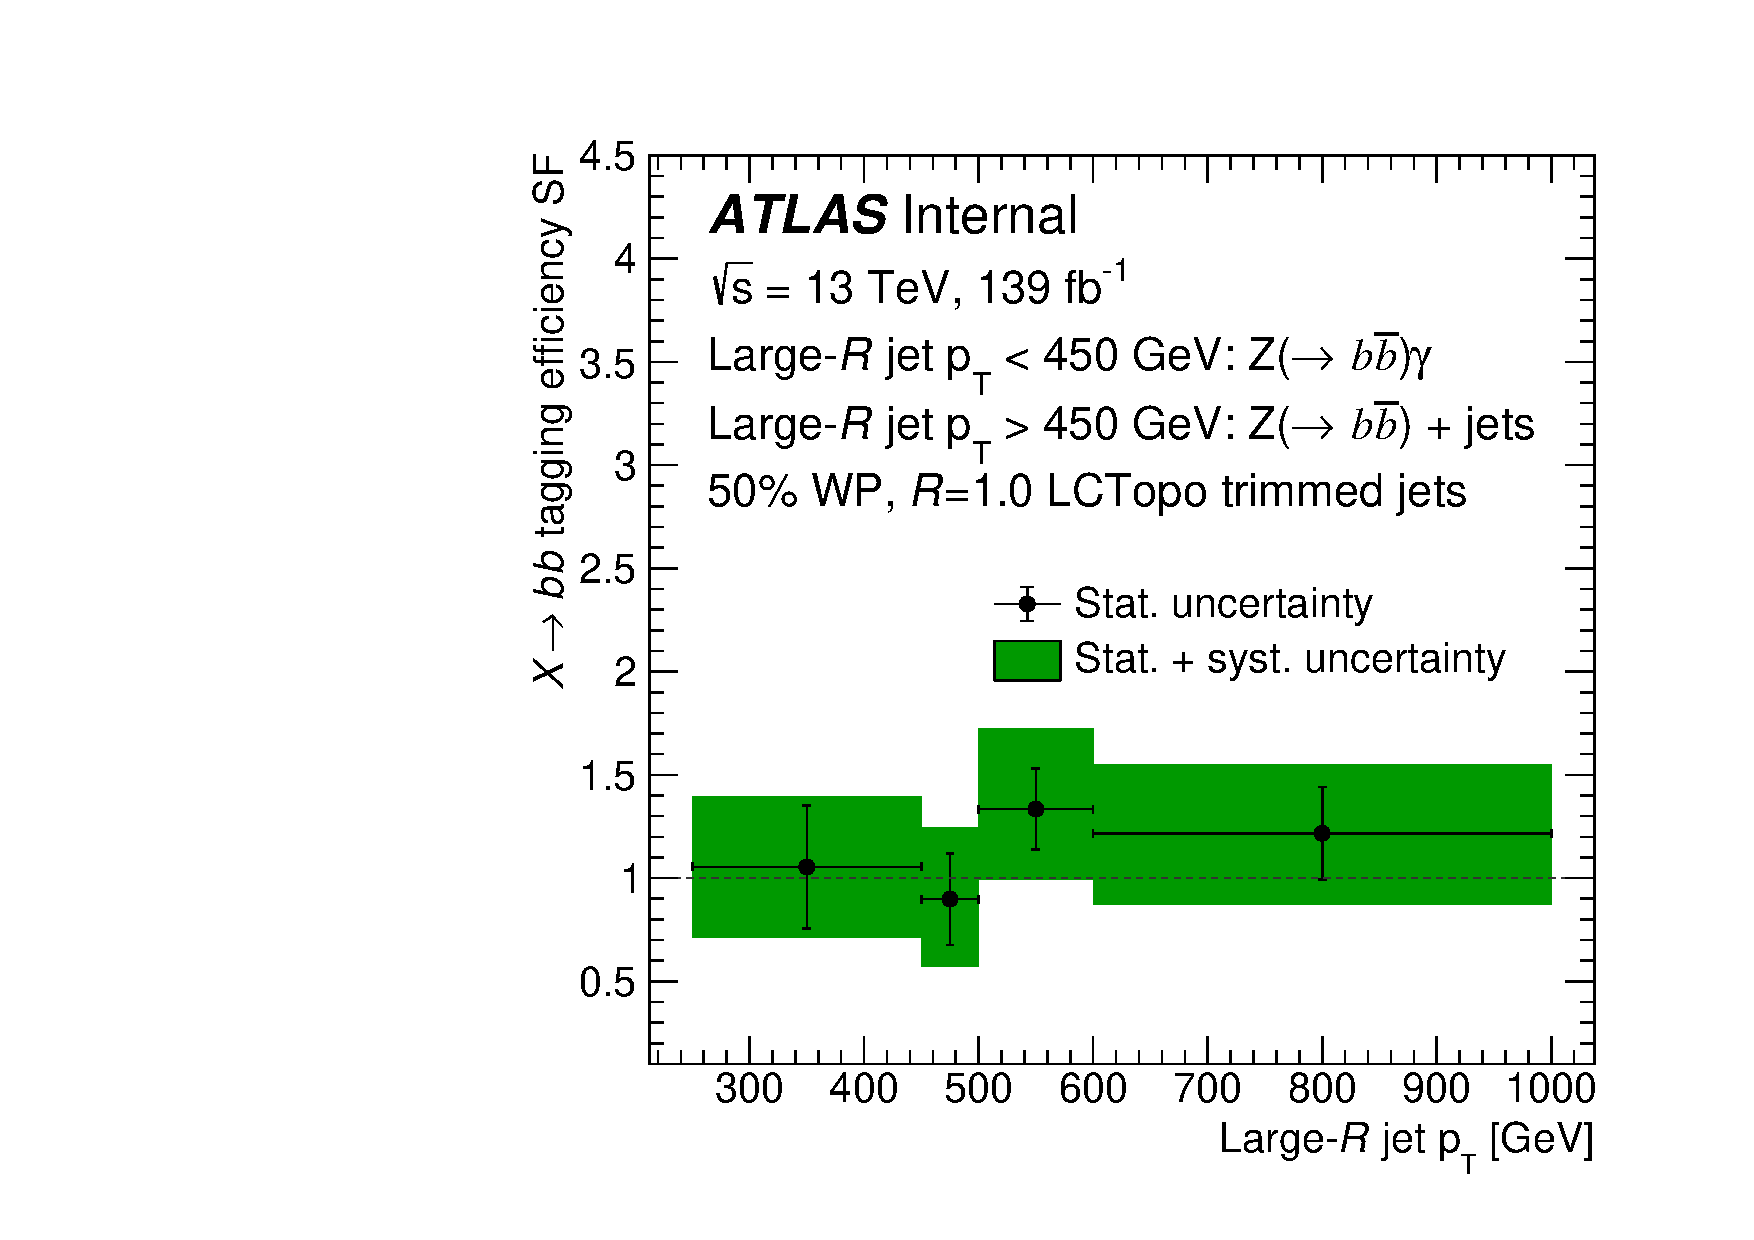
\includegraphics[width=.49\textwidth]{SF_Xbb50_internal_09March2023}}
        \subfigure[]{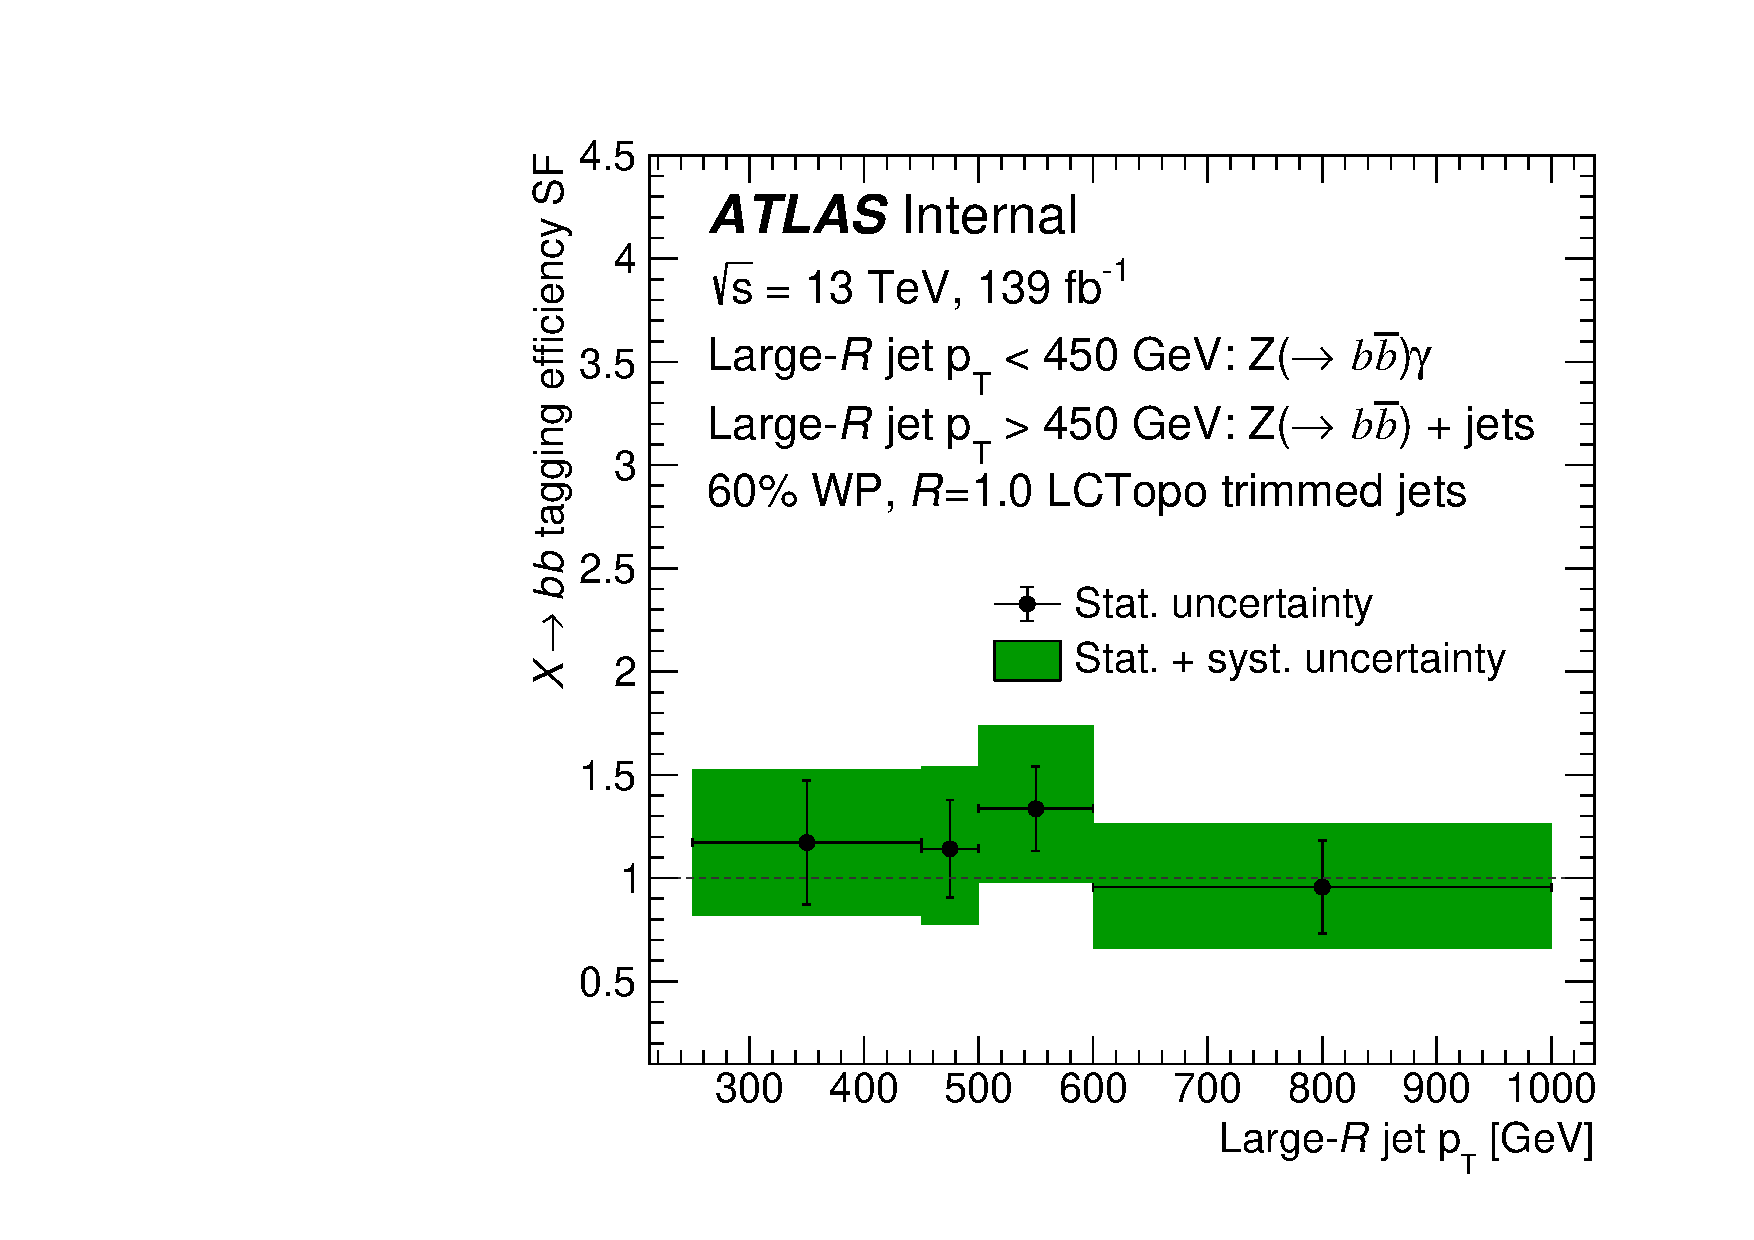
\includegraphics[width=.49\textwidth]{SF_Xbb60_internal_09March2023}} 
\caption[]{Derived scale factors in large-$R$ jet \pt for the \textbf{(a)} \qty[]{50}{\percent} and \textbf{(b)} \qty[]{60}{\percent} \ac{wp} from the calibration of the $X\rightarrow bb$ tagger.}
\label{fig:xbb_sf}    
\end{figure}

\section{Theory Uncertainties}

\section{Background Uncertainties}







theory errors
methodische errors, bkg unc

this analysis driven by stats

modelling errors

statistical unc sqrt(w) blah

luminosity

\section{Reconstruction Uncertainties}
